\documentclass{beamer}

% Theme and Color Scheme
\usetheme{Madrid}
\usecolortheme{default}

% Required Packages
\usepackage{graphicx} % For including images
\usepackage{amsmath}  % For advanced math environments
\usepackage{booktabs} % For professional tables

% Title Page Information
\title{RMSTSS: A Comprehensive Software Suite for Power and Sample Size Calculation in Modern Clinical Trials}
\author{Arnab Aich, Yuan Zhang}
\institute{Department of Preventive Medicine, UTHSC}
\date{\today}

\begin{document}

% Frame 1: Title Page
\begin{frame}
  \titlepage
\end{frame}

% --- Part 1: Introduction & Foundations ---
\section{Introduction \& Foundations}

% Frame 2: The Fundamental Goal of this Project
\begin{frame}
\frametitle{The Fundamental Goal: Planning Better Clinical Trials}
Every clinical trial must answer two critical questions before it begins:

\begin{enumerate}
    \item \textbf{How many patients do we need?} (Sample Size Calculation)
    \item \textbf{What is our chance of detecting a real treatment effect?} (Statistical Power)
\end{enumerate}

\vspace{1em}

\begin{block}{Why is this relevant?}
\begin{itemize}
    \item \textbf{Ethical Responsibility:} Avoid exposing patients to ineffective treatments or running underpowered studies that cannot yield meaningful results.
    \item \textbf{Resource Allocation:} Clinical trials are expensive. Proper planning ensures efficient use of time, funding, and patient participation.
    \item \textbf{Scientific Rigor:} A well-powered study is essential for drawing valid and reliable conclusions about a treatment's efficacy.
\end{itemize}
\end{block}
\end{frame}

% Frame 3: The Standard Approach: Survival Models
\begin{frame}
\frametitle{The Standard Approach: Survival Models}
In many trials, the outcome is the \textbf{time until an event} occurs (e.g., recovery, disease progression, death).

\begin{block}{Key Notations}
\begin{itemize}
    \item $T$: The true time-to-event for a subject.
    \item $C$: The censoring time (e.g., end of study, patient drops out).
    \item We observe $Y = \min(T, C)$ and an event indicator $\delta$.
    \item \textbf{Survival Function}, $S(t) = P(T > t)$: The probability of surviving past time $t$.
    \item \textbf{Hazard Function}, $h(t)$: The instantaneous risk of the event at time $t$, given survival up to $t$.
    $$h(t) = \lim_{\Delta t \to 0} \frac{P(t \le T < t + \Delta t \mid T \ge t)}{\Delta t}$$
\end{itemize}
\end{block}
Traditionally, the treatment effect is quantified by the \textbf{Hazard Ratio (HR)}.
\end{frame}

% Frame 4: The Proportional Hazards (PH) Assumption
\begin{frame}
\frametitle{The Proportional Hazards (PH) Assumption}
The Cox model and the Hazard Ratio rely on a critical assumption: \textbf{Proportional Hazards}.

\begin{block}{What does this mean?}
The hazard in the treatment group is a constant multiple of the hazard in the control group at all points in time.
$$h_1(t) = h_0(t) \cdot \theta$$
This implies the treatment provides a \textbf{constant relative risk reduction} throughout the entire study.
\end{block}

\begin{columns}
\begin{column}{0.5\textwidth}
    \textbf{When PH Holds:}
    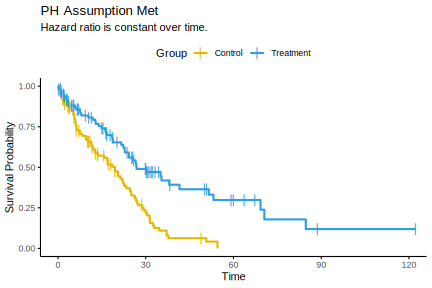
\includegraphics[width=\textwidth]{images/ph_assumption_met.png}
\end{column}
\begin{column}{0.5\textwidth}
    \textbf{When PH is Violated:}
    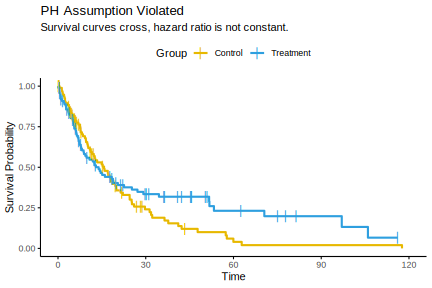
\includegraphics[width=\textwidth]{images/ph_assumption_violated.png}
\end{column}
\end{columns}
\end{frame}

% Frame 5: Problems with the Hazard Ratio
\begin{frame}
\frametitle{Problems with the Hazard Ratio}
\begin{enumerate}
    \item \textbf{The PH Assumption is Often Violated} \cite{[1]}
    \begin{itemize}
        \item Modern therapies (e.g., immunotherapies) often have \textbf{delayed effects}.
        \item Treatment benefits may \textbf{wear off} over time.
        \item This leads to \textbf{crossing survival curves}, a clear violation of the PH assumption.
    \end{itemize}
    \vspace{1em}
    \item \textbf{Lack of a Clear Causal Interpretation}
    \begin{itemize}
        \item When the PH assumption fails, the single HR value from a Cox model becomes a complex, time-averaged summary.
        \item It loses its clear meaning as a constant relative risk, making it difficult to interpret the true clinical benefit \cite{[1]}.
    \end{itemize}
\end{enumerate}
\end{frame}

% Frame 6: The Solution: Restricted Mean Survival Time (RMST)
\begin{frame}
\frametitle{The Solution: Restricted Mean Survival Time (RMST)}
\begin{block}{Definition}
The RMST is the average event-free survival time up to a pre-specified time point, $L$. It is the area under the survival curve from 0 to $L$ \cite{[1]}.
$$\mu(L) = E = \int_0^L S(t) dt$$
\end{block}

\begin{block}{Interpretation \& Advantages}
\begin{itemize}
    \item \textbf{Directly Interpretable:} It provides a clear, absolute measure of survival in units of time (e.g., "an average of 3 months of additional survival over 5 years") \cite{[1, 1]}.
    \item \textbf{No Proportional Hazards Assumption:} The RMST is a non-parametric measure, making it a valid and robust choice even when survival curves cross \cite{[1]}.
    \item \textbf{Clinically Meaningful:} It quantifies the average time gained or lost, which is highly relevant to both clinicians and patients \cite{[1]}.
\end{itemize}
\end{block}
\end{frame}

% Frame 7: Causal Interpretation of the RMST Difference
\begin{frame}
\frametitle{Causal Interpretation of the RMST Difference}
The treatment effect is quantified as the difference in RMST between the two arms. This is a clear and collapsible causal estimand.

\begin{block}{The Causal Estimand}
$$\Delta(L) = \mu_{\text{treatment}}(L) - \mu_{\text{control}}(L)$$
\end{block}

\begin{columns}
\begin{column}{0.5\textwidth}
\textbf{Interpretation:}
\begin{itemize}
    \item $\Delta(L)$ represents the \textbf{average gain in event-free time} attributable to the treatment over the time period $[0, L]$.
    \item This provides a direct answer to the question: "On average, how much longer did patients on the new treatment live without an event during the study period?"
\end{itemize}
\end{column}
\begin{column}{0.5\textwidth}
\includegraphics[width=\textwidth]{images/rmst_causal_plot.png}
\end{column}
\end{columns}
\end{frame}

% Frame 5: Direct Regression Modeling of RMST
\begin{frame}
\frametitle{Direct Regression Modeling of RMST}
Instead of estimating survival curves first, we can model the RMST directly as a function of covariates, $Z_i$.

\begin{block}{The General Model Structure}
$$g(E[\mu_i | Z_i]) = \beta_0 + \beta'Z_i$$
\end{block}
\begin{itemize}
    \item $\mu_i$ is the RMST for subject $i$.
    \item $Z_i$ is a vector of covariates (e.g., treatment arm, age, biomarkers).
    \item $g(\cdot)$ is a link function (e.g., identity for additive effects, log for multiplicative effects).
\end{itemize}
\vspace{1em}
\textbf{Handling Censoring}:
\begin{itemize}
    \item These models use \textbf{Inverse Probability of Censoring Weighting (IPCW)} to correct for right-censoring, providing unbiased estimates of the $\beta$ coefficients \cite{[1]}.
\end{itemize}
\end{frame}

% --- Part 2: The RMSTSS Package: Models & Methods ---
\section{The RMSTSS Package: Models \& Methods}

% Frame 6: The RMSTSS R Package Ecosystem
\begin{frame}
\frametitle{The `RMSTSS` R Package Ecosystem}
`RMSTSS` is designed to bridge the gap between advanced statistical methods and practical trial design \cite{[1]}. It consists of two main components:
\begin{enumerate}
    \item \textbf{The R Package}: A powerful, scriptable backend for statisticians and methodologists who need flexibility and reproducibility.
    \item \textbf{The Shiny Application}: An intuitive, graphical frontend for a broader audience of researchers and clinicians who prefer a no-code solution.
\end{enumerate}
\end{frame}

% Frame 7: Core Computational Approaches
\begin{frame}
\frametitle{Core Computational Approaches}
`RMSTSS` offers two distinct methods for calculation, allowing users to balance speed and robustness \cite{[1]}.

\begin{block}{1. Analytic (`.analytical`)}
\begin{itemize}
    \item \textbf{How it works}: Uses a direct mathematical formula based on the asymptotic variance of the treatment effect.
    $$\text{Power} = \Phi\left( \frac{|\beta_{\text{effect}}|}{\sigma_N} - z_{1-\alpha/2} \right)$$
    \item \textbf{Advantages}: Extremely fast, ideal for quickly exploring multiple design scenarios.
\end{itemize}
\end{block}

\begin{block}{2. Bootstrap (`.boot`)}
\begin{itemize}
    \item \textbf{How it works}: A robust, simulation-based method that repeatedly resamples from the pilot data.
    $$\text{Power} = \frac{\text{Number of simulations with } p < \alpha}{n_{\text{sim}}}$$
    \item \textbf{Advantages}: Makes fewer distributional assumptions, highly robust.
\end{itemize}
\end{block}
\end{frame}

% Frame 8: Model 1: Linear IPCW Model
\begin{frame}
\frametitle{Model 1: Linear IPCW Model}
\begin{block}{Use Case}
Standard trial designs where a linear relationship between covariates and RMST is assumed. Based on Tian et al. (2014) \cite{[1]}.
\end{block}

\begin{block}{Mathematical Model}
The conditional RMST is modeled as a linear function of covariates $Z_i$:
$$E = \beta_0 + \beta' Z_i$$
\end{block}
\end{frame}

% Frame 9: Estimation for Linear Model: IPCW
\begin{frame}
\frametitle{Estimation for Linear Model: IPCW}
\begin{block}{The Challenge of Censoring}
We observe $Y_i = \min(T_i, C_i)$ and an event indicator $\delta_i$. We cannot directly regress $Y_i$ on $Z_i$.
\end{block}

\begin{block}{The IPCW Solution}
\begin{itemize}
    \item Let $G(t) = P(C_i > t)$ be the survival function of the censoring time.
    \item The weight for an uncensored subject ($\delta_i=1$) is the inverse of the probability of not being censored by their event time:
    $$w_i = \frac{\delta_i}{\hat{G}(Y_i)}$$
    \item $\hat{G}(t)$ is estimated using the Kaplan-Meier method on the censoring distribution.
    \item A standard weighted least squares regression is then fitted.
\end{itemize}
\end{block}
\end{frame}

% Frame 10: Model 2: Stratified Models for Multi-Center Trials
\begin{frame}
\frametitle{Model 2: Stratified Models for Multi-Center Trials}
\begin{block}{Use Case}
Trials with a large number of strata, such as clinical centers, where estimating a separate parameter for each stratum is inefficient \cite{[1]}.
\end{block}
Two main approaches are supported:
\begin{itemize}
    \item \textbf{Additive Model}: Assumes a constant treatment benefit across strata.
    \item \textbf{Multiplicative Model}: Assumes a proportional treatment benefit across strata.
\end{itemize}
\end{frame}

% Frame 11: Additive Stratified Model
\begin{frame}
\frametitle{Additive Stratified Model}
\begin{block}{Use Case}
The treatment is expected to add a constant amount of survival time across all strata. Based on Zhang et al. (2024) \cite{[1]}.
\end{block}
\begin{block}{Mathematical Model}
The model allows each stratum $j$ to have its own baseline RMST ($\mu_{0j}$), with a common treatment effect $\beta$:
$$\mu_{ij} = \mu_{0j} + \beta'Z_i$$
\end{block}
\begin{block}{Estimation}
The common effect $\beta$ is estimated efficiently via a \textbf{stratum-centering} approach on the IPCW-weighted data, which avoids direct estimation of the numerous $\mu_{0j}$ parameters.
\end{block}
\end{frame}

% Frame 12: Multiplicative Stratified Model
\begin{frame}
\frametitle{Multiplicative Stratified Model}
\begin{block}{Use Case}
The treatment is expected to multiply survival time proportionally across strata. Based on Wang et al. (2019) \cite{[1]}.
\end{block}
\begin{block}{Mathematical Model}
The covariates have a multiplicative effect on the stratum-specific baseline RMST:
$$\mu_{ij} = \mu_{0j} \exp(\beta'Z_i)$$
This is equivalent to a linear model on the log-RMST:
$$\log(\mu_{ij}) = \log(\mu_{0j}) + \beta'Z_i$$
\end{block}
\begin{block}{Estimation}
The package uses a practical and efficient approximation by fitting a weighted log-linear model.
\end{block}
\end{frame}

% Frame 13: Model 3: Semiparametric GAM Model
\begin{frame}
\frametitle{Model 3: Semiparametric GAM Model}
\begin{block}{Use Case}
When a covariate, such as age or a biomarker level, is expected to have a non-linear effect on the RMST \cite{[1]}.
\end{block}
\begin{block}{Mathematical Model}
A Generalized Additive Model (GAM) is used, modeling non-linear relationships with smooth functions (splines), $f_k()$:
$$ E[\text{pseudo}_i] = \beta_0 + \beta_1 \cdot \text{Treatment}_i + \sum_{k=1}^{q} f_k(\text{Covariate}_{ik}) $$
\end{block}
\end{frame}

% Frame 14: Estimation for GAM Model: Pseudo-Observations
\begin{frame}
\frametitle{Estimation for GAM Model: Pseudo-Observations}
\begin{block}{The Challenge}
Standard regression models like GAMs cannot directly handle censored time-to-event data.
\end{block}
\begin{block}{The Solution: Jackknife Pseudo-Observations}
\begin{enumerate}
    \item The time-to-event outcome is converted into a continuous, uncensored variable called a **pseudo-observation**.
    \item Let $\hat{\mu}$ be the RMST estimated from the full sample of size $n$, and $\hat{\mu}_{(-i)}$ be the RMST estimated from the sample with subject $i$ removed.
    \item The pseudo-observation for subject $i$ is:
    $$\text{pseudo}_i = n \cdot \hat{\mu} - (n-1) \cdot \hat{\mu}_{(-i)}$$
    \item The GAM is then fitted to these pseudo-observations.
\end{enumerate}
\end{block}
\end{frame}

% Frame 15: Model 4: Dependent Censoring Model
\begin{frame}
\frametitle{Model 4: Dependent Censoring Model}
\begin{block}{Use Case}
Studies with competing risks, where censoring may not be independent of the event of interest (e.g., receiving a transplant precludes pre-transplant death). Based on Wang et al. (2018) \cite{[1]}.
\end{block}
\begin{block}{Mathematical Model}
The final analysis still uses a weighted linear model for the RMST:
$$E = \beta_0 + \beta' Z_i$$
However, the calculation of the IPCW weights is extended to handle the dependent censoring.
\end{block}
\end{frame}

% Frame 16: Estimation for Dependent Censoring Model
\begin{frame}
\frametitle{Estimation for Dependent Censoring Model}
\begin{block}{The Challenge}
A single censoring distribution is no longer sufficient.
\end{block}
\begin{block}{The Solution: Cause-Specific Weights}
\begin{itemize}
    \item Instead of one model for the overall censoring distribution, **cause-specific Cox models** are fitted for each of the $K$ sources of censoring.
    \item The final weight for a subject is a product of the weights derived from all censoring causes, calculated as \cite{[1]}:
    $$W_i = \exp\left(\sum_{k=1}^{K} \hat{\Lambda}_{k}(Y_i)\right)$$
    where $\hat{\Lambda}_{k}$ is the estimated cumulative hazard for censoring cause $k$.
\end{itemize}
\end{block}
\end{frame}

% Frame 17: Package Functionality & Naming
\begin{frame}
\frametitle{Package Functionality \& Naming}
The package uses a consistent and predictable `model.goal.method` naming convention, making it easy to find the right function.
\begin{itemize}
    \item \textbf{Choose a `model`}: \texttt{linear}, \texttt{additive}, \texttt{MS}, \texttt{GAM}, \texttt{DC}
    \item \textbf{Choose a `goal`}:
    \begin{itemize}
        \item \texttt{power}: To calculate power for given sample sizes.
        \item \texttt{ss}: To find the sample size for a target power.
    \end{itemize}
    \item \textbf{Choose a `method`}:
    \begin{itemize}
        \item \texttt{analytical}: For the fast, formula-based approach.
        \item \texttt{boot}: For the robust, simulation-based approach.
    \end{itemize}
\end{itemize}
\vspace{1em}
\textbf{Example}: To find the \textbf{s}ample \textbf{s}ize for the \textbf{m}ultiplicative \textbf{s}tratified model using the \textbf{boot}strap method, you would call \texttt{MS.ss.boot()}.
\end{frame}

% Frame 18: Using the R Package: An Example
\begin{frame}[fragile]
\frametitle{Using the R Package: An Example}
Calculating the required sample size for a multi-center trial using the additive stratified model is straightforward.

\begin{block}{Scenario}
Using the `colon` dataset, we want to find the sample size per stratum (`extent`) to achieve 80\% power, with a truncation time of 5 years (1825 days).
\end{block}

\begin{block}{R Code}
\begin{verbatim}
# Load and prepare data
library(survival)
library(RMSTSS)
colon_death <- colon[colon$etype == 2, ] %>% 
  na.omit()
colon_death$arm <- ifelse(colon_death$rx == "Obs", 0, 1)
colon_death$strata <- factor(colon_death$extent)

# Run the sample size calculation
ss_results <- additive.ss.analytical(
  pilot_data = colon_death,
  time_var = "time", status_var = "status", 
  arm_var = "arm", strata_var = "strata", 
  target_power = 0.80, L = 1825
)

# View results and plot
print(ss_results$results_data)
\end{verbatim}
\end{block}
\end{frame}

% --- Part 3: The RMSTSS Shiny Application ---
\section{The RMSTSS Shiny Application}

% Frame 19: The `RMSTSS` Shiny Application
\begin{frame}
\frametitle{The `RMSTSS` Shiny Application}
The Shiny application makes the full power of the `RMSTSS` package accessible through an intuitive graphical interface \cite{[1]}.

\textbf{Key Features} \cite{[1]}:
\begin{itemize}
    \item \textbf{Easy Data Upload}: Start by uploading your pilot data in a standard `.csv` format.
    \item \textbf{Visual Column Mapping}: Use dropdown menus to map your data columns to the required model variables.
    \item \textbf{Point-and-Click Analysis}: Select your desired model, goal, and all relevant parameters without writing any code.
    \item \textbf{Interactive Outputs}: Immediately visualize results, including survival curves and the final power curve.
    \item \textbf{One-Click Reporting}: Generate a comprehensive, publication-ready PDF or HTML report that documents your analysis.
\end{itemize}
\end{frame}

% Frame 20: Application Screenshot
\begin{frame}
\frametitle{Application Interface}
\begin{figure}
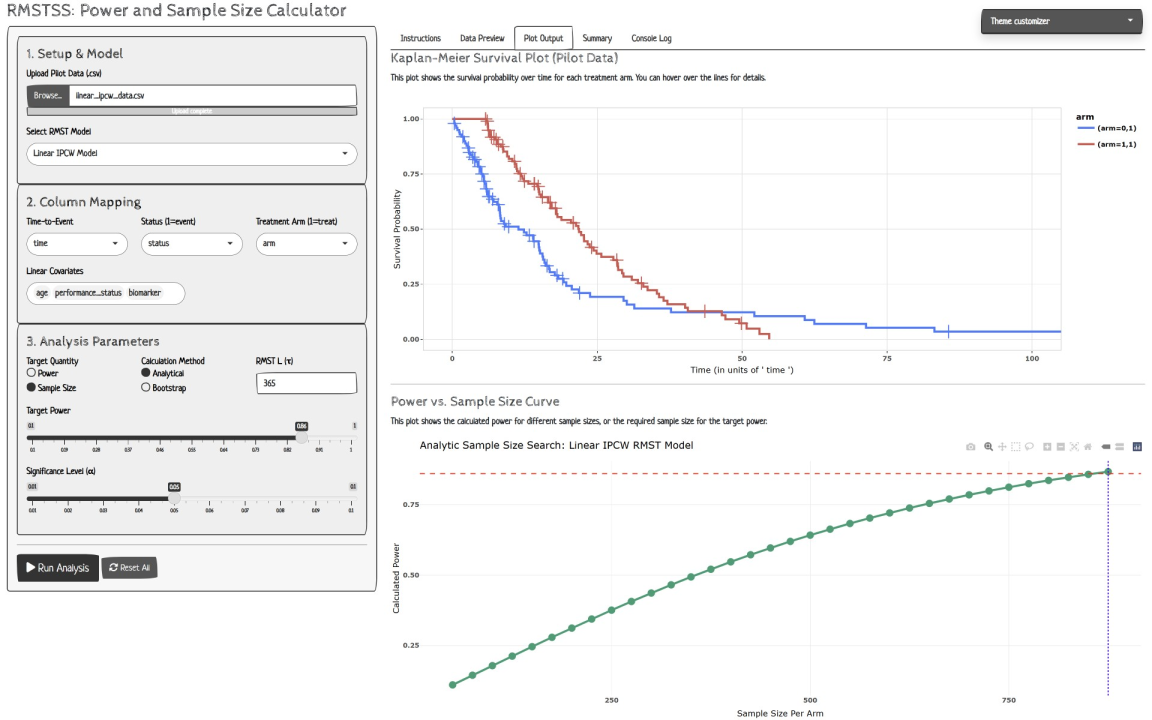
\includegraphics[width=\textwidth]{images/app-ss.png}
\caption{The main analysis panel of the Shiny application, showing the user interface for model selection and result visualization.}
\end{figure}
\end{frame}

% Frame 21: Conclusion
\begin{frame}
\frametitle{Conclusion}
\textbf{`RMSTSS` provides a powerful, flexible, and accessible software suite for designing modern clinical trials.}
\begin{itemize}
    \item \textbf{Statistically Rigorous}: Implements a wide range of modern, direct-regression RMST models.
    \item \textbf{Causally Meaningful}: Empowers researchers to design trials based on the highly interpretable RMST endpoint.
    \item \textbf{Accessible to All}: Caters to both expert statisticians via the R package and a broader research community via the Shiny application.
\end{itemize}
\end{frame}

% Frame 22: Access & Acknowledgments
\begin{frame}
\frametitle{Access \& Acknowledgments}
\textbf{Access the Software}:
\begin{itemize}
    \item \textbf{Live Web App}: \texttt{arnab96.shinyapps.io/uthsc-app/}
    \item \textbf{R Package on GitHub}: \texttt{github.com/arnab-aich/RMSTSS}
\end{itemize}
\vspace{1em}
\textbf{Acknowledgments} \cite{[1]}:
\begin{itemize}
    \item NSF grant no. 2220726.
    \item UTHSC BERD (Biostatistics, Epidemiology and Research Design).
\end{itemize}
\vfill
\begin{center}
\Huge{\textbf{Questions?}}
\end{center}
\end{frame}

\end{document}
